% https://www.youtube.com/watch?v=fCzF5gDy60g
% https://www.youtube.com/playlist?list=PLknjcpwMhvSgauKyhScPiQGW9H4V0EKj5

% Preamble
\documentclass[12pt]{DistributedDatabases}[2021/12/09]

\usepackage{hyperref}
\usepackage{graphicx}

% Document Environment
\begin{document}

\frontmatter % Use roman page numbering style (i, ii, iii, iv...) for the pre-content pages

\begin{titlepage}
\begin{center}

\vspace*{.06\textheight}
{\scshape\LARGE{Hogeschool Gent}}
\vspace{1.5cm}

\HRule \\[0.8cm] % Horizontal line
{\huge{Distributed Databases}}\vspace{0.4cm}
\HRule \\[1.5cm] % Horizontal line

\vfill

\large \textit{\textbf{Machine Learning}}\\[0.4cm]
\textit{\textbf{with}}\\[0.4cm]
\textit{\textbf{auto-sklearn}}\\[0.4cm]

\vfill

\begin{flushright} \large
  \emph{Students}\\
  Wim \textsc{Suenens} \\
  Bazille \textsc{Van de Walle} \\
  \vspace{1.0cm}
  \emph{Professor}\\
  Stijn \textsc{Lievens}
\end{flushright}

\vfill

{\large \today}\\[2cm]

\vfill
\end{center}
\end{titlepage}

\tableofcontents
% \listoffigures
% \listoftables

\mainmatter % Begin numeric (1,2,3...) page numbering
% \newpage
\setcounter{page}{1}


\chapter{Introduction}
\lipsum[2-2]

\chapter{Regression}
In this section we discuss the datasets we used to research regression.
We will explain in greater detail how our model performed, compare it to other models on and give some info over the dataset.

\section{Used Car Prices}
For this dataset we used the competition version of the big data set provided on Kaggle. This set is based on a big dataset of 100 000 listings on used cars in the UK. We then found and used a version that was slimmed down for competition. This dataset looked ideal for us to learn more about auto-sklearn.
\\
\url{https://www.kaggle.com/adityadesai13/used-car-dataset-ford-and-mercedes?select=vw.csv}
\url{https://www.kaggle.com/kukuroo3/used-car-price-dataset-competition-format}

\subsection{Dataset}

The dataset is based on a list of 100 000 listings of used cars in the UK.
This dataset was preprocessed and separated into competition format.
The label for the test data is provided in the form of a function.
After cleaning the data we where left with the following columns:
\\
carID, brand ,model year, transmission, mileage, fuelType, tax, mpg, engineSize, price.
Their are 2672 entries in total.
\subsection{Model Performance}

First we visualised the dataset with 2 different pairplots.
This gave us an idea of what to expected from this dataset.
The pairplot that is based on the fueltype shows clearly that petrol cars are the most common.
\begin{figure}
    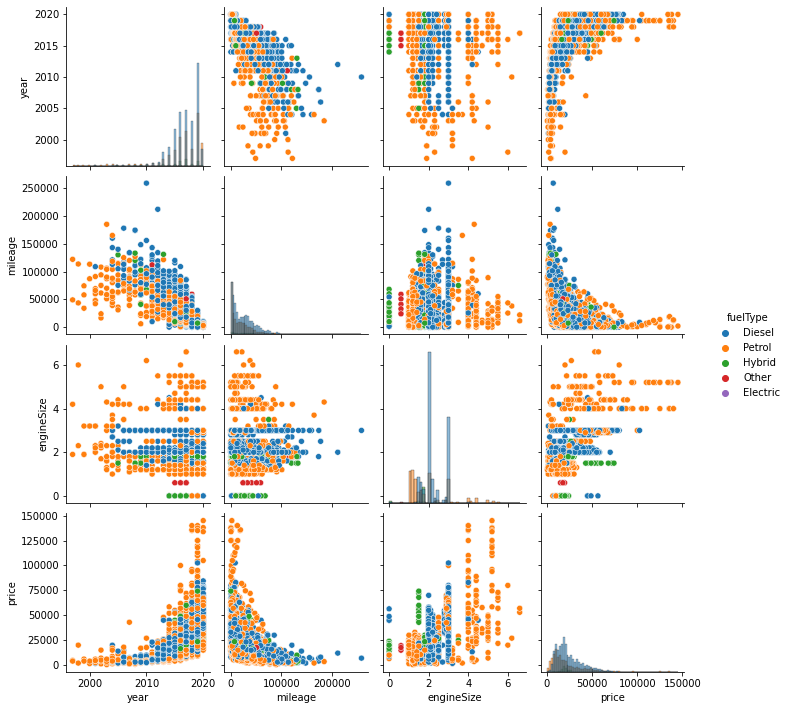
\includegraphics[width=\linewidth]{images/pairplot_fueltype.png}
    \caption{A pairplot based on fueltype}
    \label{fig:pairplot fueltype}
\end{figure}
The pairplot that is based on the brand shows clearly that the german brands are most common.
\begin{figure}
    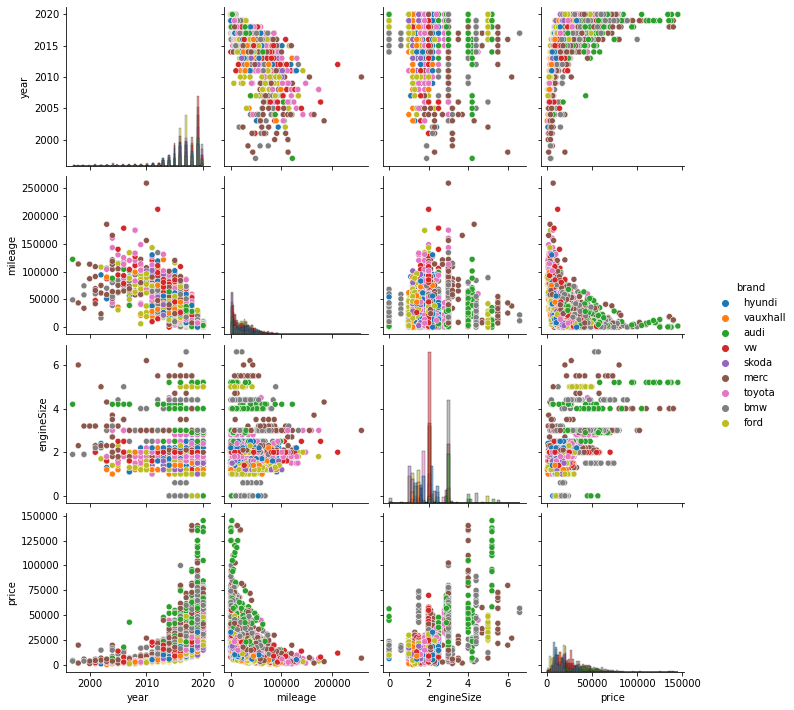
\includegraphics[width=\linewidth]{images/pairplot_brand.png}
    \caption{A pairplot based on brand}
    \label{fig:pairplot brand}
\end{figure}
\\
After fitting and training the data this are the results we got for the different data sets.

\begin{table}[h!]
    \begin{center}
        \caption{Table with training results.}
        \label{tab:training results}
        \begin{tabular}{l|S|r|l} % <-- Changed to S here.
            \textbf{function} & \textbf{Training data} & \textbf{Test data} & \textbf{Validation data}\\
            \hline
            mean squared error & 59050.4794 & 293230.5317 & 585230.4846\\
            mean absolute error & 26.3980 & 55.7094 & 59.8129\\
            r2 & 0.9998 & 0.9989 & 0.9979\\
        \end{tabular}
    \end{center}
\end{table}

\subsection{Model Comparision}

We chose 3 models from kaggle to compare our results with. After comparing our scores we found out that we have a better performing model. Our model included te model of the car, this was something the other models left out. We can conclude that our models performs better than the ones we compared scores with.
\\
Url1: \url{https://www.kaggle.com/selinsong/u-car-rf-r2-score-0-94/data}

Url2: \url{https://www.kaggle.com/yuyuyuyuy/rf-test-r2-score-0-956}

Url3: \url{https://www.kaggle.com/johyunkang/py-rf-test-r2-0-939}

\begin{table}[h!]
    \begin{center}
        \caption{Table with r2 results.}
        \label{tab:training results}
        \begin{tabular}{l|S} % <-- Changed to S here.
            \textbf{data} & \textbf{R2 score} \\
            \hline
            Training data & 0.9997784238195022\\
            Test data & 0.9989334899119373 \\
            Validation data & 0.9978756073515518\\
            Url1 & 0.94\\
            Url2 & 0.956\\
            Url3 & 0.939\\
        \end{tabular}
    \end{center}
\end{table}

\section{Television Brand E-commerce}
This dataset can be used to explore the current market scenario for Televisions. There are various types of screens with different operating systems offered by several manufacturers at competitive prices.

\subsection{Dataset}
This dataset includes specifications of different televisions offered by various brands with prices and ratings.
It contains 912 samples with 7 attributes. Here are the columns in this dataset-
Brand Resolution Size Selling Price Original Price Operating System Rating

Brand: This indicates the manufacturer of the product i.e. Television
Resolution: This has multiple categories and indicates the type of display i.e. LED, HD LED, etc.
Size: This indicates the screen size in inches
Selling Price: This column has the Selling Price or the Discounted Price of the product
Original Price: This includes the Original Price of the product from the manufacturer.
Operating system: This categorical variable shows the type of OS like Android, Linux, etc.
Rating: Average customer ratings on a scale of 5.

\subsection{Model Performance}
First we visualised the dataset with a pairplot.
This gave us an idea of what to expected from this dataset.
The pairplot that is based on the resolution shows clearly HD LED and ULTRA HD LED are the most common resolution.
\begin{figure}
    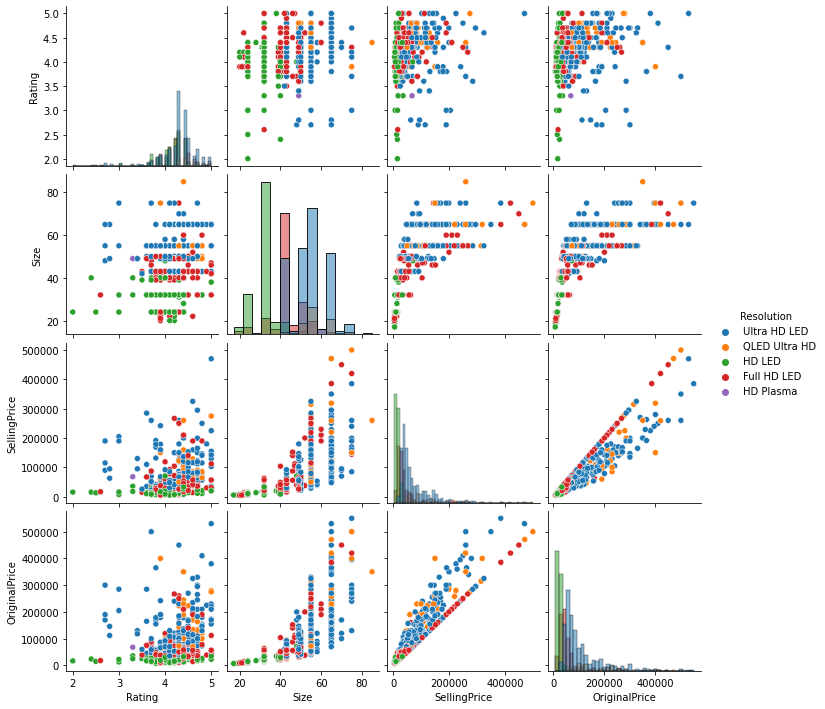
\includegraphics[width=\linewidth]{images/pairplot_resolution.png}
    \caption{A pairplot based on tv resolution}
    \label{fig:pairplot resolution}
\end{figure}

After fitting and training the data this are the results we got for the different data sets.

\begin{table}[htp]
    \begin{center}
        \caption{Table with training results.}
        \label{tab:training results}
        \begin{tabular}{l|S|r} % <-- Changed to S here.
            \textbf{function} & \textbf{Training data} & \textbf{Test data} \\
            \hline
            mean squared error & 81016219.59417547 & 952681194.3707451 \\
            mean absolute error & 5251.913730638445 & 14205.972881317139 \\
            r2 & 0.9796709758590545 & 0.8247644898857763\\
        \end{tabular}
    \end{center}
\end{table}

\subsection{Model Comparision}
When we looked on the kaggle page of this dataset we found out that there are not yet any other auto-sklearn projects submitted. Thats why we can not compare our results with someone else. We do notice te big difference between test and training data results.
Url1: \url{https://www.kaggle.com/devsubhash/television-brands-ecommerce-dataset/code}
\chapter{Classification}
\newcommand{\linkAutoSklearnClassifier}{https://www.kaggle.com/andrewmvd/heart-failure-clinical-data}

Within auto-sklearn, we can make use of the \href{\linkAutoSklearnClassifier}{'AutoSklearnClassifier'\footnote{AutoSklearnClassifier: \href{\linkAutoSklearnClassifier}{\linkAutoSklearnClassifier}}} to implement a model for a classifcation problem.

\section{Heart Failure Prediction}
\label{HeartFailurePrediction}

The first classification problem we discuss is about the prediction of heart failure based upon different parameters.

\subsection{Dataset}
\newcommand{\kagglelinkheartfailure}{https://www.kaggle.com/andrewmvd/heart-failure-clinical-data}

The \href{\kagglelinkheartfailure}{dataset\footnote{Heart Failure Prediction : \href{\kagglelinkheartfailure}{\kagglelinkheartfailure}}} can be found on Kaggle and contains 12 features which can be used to predict mortality by heart failure. Those features are:

\begin{itemize}
  \item age: The age of the person in the dataset.
  \item anaemia: Whether the person has a decrease of red blood cells or hemoglobin ($boolean$).
  \item creatinine\_phosphokinase: The level of the CPK enzyme in the blood ($mcg/L$).
  \item diabetes: Whether the patient has diabetes ($boolean$).
  \item ejection\_fraction: The percentage of blood leaving the heart at each contraction ($percentage$).
  \item high\_blood\_pressure: Whether the patient suffers from hypertension ($boolean$).
  \item platelets: The number of platelets in the blood ($kiloplatelets/mL$).
  \item serum\_creatinine: The level of serum creatinine in the blood ($mg/dL$).
  \item serum\_sodium: The level of serum sodium in the blood ($mEq/L$).
  \item sex: woman or man ($binary$).
  \item smoking: Whether the patient smokes or not ($boolean$).
  \item time: Follow-up period ($days$)
\end{itemize}

\noindent There are 299 observations in the dataset. For none of the features data is missing.

\subsection{Model Performance}

To construct the model, we've taken 30\% out of the dataset for testing purposes. The remaining part will be used to build our model with a $random\_state$ of 42. After fitting the model with the training data we can measure the performance of the model on the training and testing data. On the training data the model scores an accuracy of 96,17\%.

The mean accuracy reduces for the testing data to 73,33\%. When we compare the actual testing labels with the predicitons of the model for the testing data, we get a accuracy score of 73,33\%, with a precision of 78,26\%

\begin{figure}[t]
  \begin{center}
    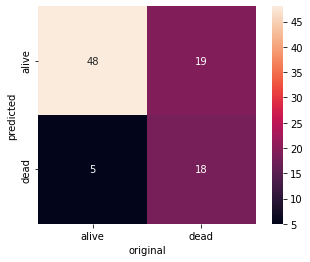
\includegraphics{heart-failure-heatmap}
    \caption{Heatmap of the confusion matrix for the heart failure predicitons}
  \end{center}
  % \centering
\end{figure}


\subsection{Model Comparision}

When we check the previous kaggle submissions with the same dataset, we can see the use of a LogisticRegression model from sklearn by '\href{https://www.kaggle.com/manthannagpurkar/heart-failure-prediction}{manthannagpurkar}' can improve the accuracy on the testing data up to 80\%.


\section{Diabetes Prediction}
\newcommand{\linkLogisticRegression}{https://scikit-learn.org/stable/modules/generated/sklearn.linear\_model.LogisticRegression.html}
\newcommand{\linkGaussianNB}{https://scikit-learn.org/stable/modules/generated/sklearn.naive\_bayes.GaussianNB.html?highlight=gaussiannb}
\newcommand{\linkRandomForestClassifier}{https://scikit-learn.org/stable/modules/generated/sklearn.ensemble.RandomForestClassifier.html?highlight=randomforestclassifier}



As a fourth model and as a comparision with the outcome during the lectures, we've choosen the 'diabetes' dataset, which has been analysed by using a 'VotingClassifier' including a \href{\linkLogisticRegression}{LogisticRegression\footnote{\url{\linkLogisticRegression}}}, a \href{\linkGaussianNB}{GaussianNaiveBayes\footnote{\url{\linkGaussianNB}}} and a \href{\linkRandomForestClassifier}{RandomForestClassifier\footnote{\url{\linkRandomForestClassifier}}}. We will use the AutoSklearnClassifier and compare it's score with the VotingClassifier.

\subsection{Dataset}

The dataset can be found on github, has 724 entries and contains 8 features. Those features are:

\begin{itemize}
  \item Pregnancies: The number of pregnancies.
  \item Glucose: The concentration of glucose after 2 hours in an oral glucose tolerance test.
  \item BloodPressure: Diastolic blood pressure ($mm Hg$).
  \item SkinThickness: Triceps skin fold thickness ($mm$).
  \item Insulin: 2-Hour serum insulin ($mu U/ml$).
  \item BMI: Body mass index ($kg/m^2$)
  \item DiabetesPedigreeFunction: likelihood of diabetes based on family history.
  \item Age: Age in years.
\end{itemize}

Similar as in lecture exercise we exclude all zero observations for 'BloodPressure', 'Glucose' and 'BMI', given these observations seem to be incorrect.

\subsection{Model Performance}

The modeling process is similar to the model for \nameref{HeartFailurePrediction}. We again use the 'AutoSklearnClassifier', after splitting the dataset into two part, a train and a test set.
After, we've fit the model with our training data, we can make the predicitons for our testing data and compare with the actual labels.
Our model get an accuracy of 87,35\% on the training data and 75,68\% on the testing data.

Comparing the actual testing labels with the predicitons of the model for the testing data, we get a accuracy score of 75,68\%. However, the precision is only 62,50\%.

\begin{figure}[t]
  \begin{center}
    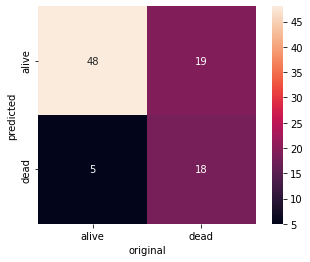
\includegraphics{heart-failure-heatmap}
    \caption{Heatmap of the confusion matrix for the diabetes predicitons}
  \end{center}
  % \centering
\end{figure}

\subsection{Model Comparision}

When we compare our model with the VotingClassifier built in the lecture exercise, we can see our model performs pretty similar. The accuracy of the VotingClassifier is 75,69\% with a precision of 62,90\%.

This is somewhat suprising as the VotingClassifier train its model on an ensemble of multiple models and can sort out the 'mistakes' of the different provided models. We can conclude the AutoSklearnClassifier can construct a model which is pretty accurate with minor effort needed.


\end{document}